\documentclass{article}
\usepackage{url}
\usepackage{amssymb,amsfonts,amsmath,amsthm,mathtools}
\usepackage{adjustbox}
\usepackage{float}
\usepackage{caption}
\usepackage{mdframed}
\usepackage{lmodern}
\usepackage{bm,bbold}
\usepackage{xfrac, nicefrac}
\usepackage{lmodern}
\usepackage{enumitem}
\usepackage[margin=60pt]{geometry}
\pdfinclusioncopyfonts=1
\captionsetup{width=0.85\textwidth}
\renewcommand{\baselinestretch}{1.5}

\include{notations}
\begin{document}
	\title{Substitution rate responses to changes in effective population size.}
	\author{T. Latrille, N. Lartillot}
	\maketitle
	
	\abstract{
		The quasi-neutral theory of evolution asserts that the effective population size ($\Ne$) plays an important role in shaping the evolution of molecular sequences.
		One consequence is that $\Ne$ modulates selection, such populations with high $\Ne$ would have stronger purifying selection, due to the decrease of random drift.
		In molecular sequence, this effect translates in the decrease in the substitution rate of selected mutations relative to the substitution rate of neutral mutation ($\dnds$) with respect to $\Ne$.
		Such theoretical prediction had been observed in empirical data across many clades.
		However, several studies failed to observe such response of $\dnds$ to changes in $\Ne$, or with weak strength or direction.
		Computational models of protein folding have observed that $\dnds$ can be independent of $\Ne$, which can mathematically be proven under certain assumptions.
		Moreover, non-equilibrium properties can imply that an increase of $\Ne$ can result first in an increase of $\dnds$ and then a decrease.
		Together, assumptions about the mapping of sequence to fitness can display a variety of behaviors in the $\dnds$ responses to changes in $\Ne$.
		Our goal in this present work is to provide theoretical tools to derive the relationship between $\Ne$ and $\dnds$ in the context of a genotype-phenotype-fitness map.
		We apply our framework in the special case of fitness proportional to the probability of protein folding.
		Our compact theoretical results are supported by more complex simulations using 3d structure of proteins.
		We assert that models based on the probability of folding are at odds with empirically results obtained on the $\Ne$-$\dnds$ relationship in population genetic dataset.
		However, our framework applied to the case of non-specific interactions between proteins suits more the empirical data.
		We also stress the importance of epistatic interactions in the $\Ne$-$\dnds$ relationship, such that it determines to time to reach a new equilibrium, and that models without epistasis might be too slow to be realistic.
	}
	
	\section*{Introduction}
	
	[Concernant l'introduction, j'ai pris la liberté de lisser directement le texte, de rajouter quelques petites phrases ici et là, pour compléter et ajuster le fil de l'argument. Il me semble pour autant que je n'ai pas trop trahi ton fil directeur, du moins dans la première partie. Sur la fin de l'intro, par contre, je pense qu'il faut remanier un peu plus. En particulier, (1) la question de l'articulation avec la question de la relation entre dnds et expression, et (2) le fait de bien terminer toute l'analyse de l'état des lieux avant d'en venir à la contribution spécifique de ce manuscrit; dans la version que tu avais proposé, ces deux aspects avaient tendance à se mélanger un peu sur la fin.]
	
	[je propose de scinder ton premier paragraphe en deux: un premier de perspective un peu plus générale sur l'enjeu de démêler les forces évolutives à partir des patterns de substitution, un deuxième qui en vient plus spécifiquement au rôle de la dérive génétique, et qui s'articule du coup plus directement avec la question de la théorie quasi-neutre (en passant, en anglais, c'est nearly-neutral, et non quasi-neutral). Du coup, concernant ce premier paragraphe-ci, il faut aller jusqu'au bout de l'argument, et j'ai rajouté deux phrases en ce sens.]
	Molecular sequences differ across species due to the particular history of DNA substitutions along their respective lineages.
	These substitutions in molecular sequences are the result of the interplay between evolutionary forces such as mutation, selection and random genetic drift.
	These forces have effects at different levels: mutations are carried by molecular sequence, selection is mediated at the level of individuals, while random genetic drift is a population effect.
	Yet, they jointly contribute to the long-term molecular evolutionary process.
	Thus, the challenge of molecular evolution is to tease out their respective contributions, based on comparative analyses.
	
	[The specific role of random drift $\to$ the nearly-neutral argument.]
	One main aspect of this challenge is to correctly evaluate the role of random drift in the long term evolutionary process.
	Population genetics theory implies that the strength of drift, due to the stochastic sampling of mutations, is less pronounced in lineage with large effective population size ($\Ne$), and as a consequence, the purification by selection of weakly deleterious mutations is more effective.
	This fundamental idea is at the core of the nearly-neutral theory of evolution.
	The nearly-neutral theory posits that a substantial fraction of mutations are weakly deleterious [d'abord expliciter cette composante importante de la théorie quasi-neutre].
	As a result, the theory predicts a decrease in the substitution rate per unit of time of selected mutations along a lineage with higher $\Ne$ \cite{Ohta1972, Ohta1992}, relative to the neutral substitution rate.
	[In its original version, the nearly-neutral theory also assumes a constant mutation rate per unit of time, but such assumption can be relaxed by normalizing the substitution rate of selected mutations by the substitution rate of neutral mutations such as to discard this confounding factor \cite{Ohta1972}. {\it pas tout à fait vrai: en fait, la théorie invoquait un effet temps de génération, qui était compensé par un effet Ne, résultant en une horloge moléculaire au niveau non-synonyme. Mais cela me parait un peu compliqué. Peut-être zapper ce point?}]
	
	The relative substitution rate of selected, relative to neutral, mutations (called $\dnds$ is this study) is a theoretical macroscopic observable in molecular sequence evolution [formulation compliquée.. is an observable quantity of the molecular evolutionary process?], at least if we can separately estimate the rate of neutral mutations in a phylogenetic or comparative context. Practically, in the case of protein-coding DNA sequences, and assuming that synonymous mutations are neutral, while those selected mutations are the non-synonymous changes affecting the amino-acid sequence, $\dnds$ can be identified with the ratio of non-synonymous over synonymous substitution rates ($dN/dS$). Thus, in practice, the nearly-neutral argument translates into a predicted decrease in $\dnds =  dN/dS$ as a function of long-term changes in $N_e$.
	
	This prediction has been more quantitatively examined under the assumption that the selective effects of mutations are drawn from a fixed distribution of fitness effects \cite{Welch2008} {\it citer également Kimura, 1979}. Be more specific here: Assuming a gamma DFE, a key result obtained in this context is an approximate allometric scaling of $dnds$ as a function of $N_e$ (i.e. $\dnds \sim N_e^{-\beta}$), where $\beta$ is the shape parameter of the DFE. In practice, DFEs are strongly leptokurtic: thus, predicts a weak negative relation between $\dnds$ and $N_e$.
	
	The context of protein coding sequences fostered another modeling approach, based on genotype-fitness map instead of distribution of fitness effects.
	In this alternative approach, the selective effect of a mutation depends on the fitnesses of both source and target amino-acids involved on the mutation \cite{Halpern1998}.
	For example, if the target amino-acid has a higher fitness than the current amino acid, the selective effect of the mutation is positive, and reciprocally negative for a lower fitness.
	Such a modeling approach predicts higher substitution rates between amino-acid with similar biochemical properties.
	More fundamentally, the fitness depends solely on the current genotype, not on the trajectory of mutations leading to this sequence.
	Even though this modeling approach differs substantially from the one assuming a fixed DFE, it also predicts a negative correlation between $\dnds$ and $\Ne$ \cite{Spielman2015a, DosReis2015}.
	
	Empirically, variation in [fluctuation is more in the short term, I would say] $\dnds$ along the branches of phylogenetic trees has been inferred using phylogenetic codon models applied to empirical sequences \cite{Yang2001, Zhang2004}. [Ici, donner un compte-rendu un peu plus exhaustif des analyses empiriques publiées au sujet de la relation dnds / Ne. Possiblement en deux temps: les analyses non intégratives: Popadin, et d'autres; puis, les approches de type coevol.]
	Subsequently, inference methods combining molecular sequences and lineage specific quantitative traits have found that $\dnds$ correlates positively with life-history traits such as longevity and body mass \cite{Lartillot2011,Weber2014}.
	Since longevity and body mass typically correlate negatively with $\Ne$, with low $\Ne$ corresponding to lineage with a large body size and extended longevity \cite{Romiguier2014}, these empirical correlations suggest a negative correlation between $\dnds$ and $\Ne$, thus confirming the theoretical prediction of the nearly-neutral theory of evolution.
	However, this correlation between $\dnds$ and life-history traits could not be replicated across all experiments, and depending on the clade or the potential biases taken into account, the correlation was found to be either not statistically significant (ref?), or even in the opposite direction (i.e. negative between $dnds$ and LHT) \cite{Figuet2016} (other refs?).
	
	Mitigated empirical evidence about the response of $\dnds$ to changes in $\Ne$ encouraged the search for alternative explanatory mechanisms \cite{Lanfear2014}.
	In this direction, one striking result was the proof that $\dnds$ is in fact predicted to be independent of $\Ne$ under very general cirumstances, namely [je propose d'être plus exhaustif sur l'ensemble des conditions des résultats de Cherry], whenever (i) the fitness is a log-concave function of a phenotype and (ii) the phenotype itself is equimutable. Equimutability states that the distribution of phenotypic changes due to mutations is independent the current phenotype of the individual \cite{Cherry1998}.
	This general theoretical argument has been invoked in the context of \textit{in silico} experiments of protein sequence evolution, assuming that proteins are under selection for their thermodynamic stability, the fitness being proportional to the folding probability of the protein \cite{Goldstein2013}. The thermodynamic stability is itself computed using a 3D structural model of the protein. These simulation experiments have led to the observation that $\dnds$ is essentially independent of $\Ne$. The explanation proposed for this result is that the distribution of changes in free energy of folding ($\deltadeltaG$) due to mutations is approximately independent of the current free energy ($\deltaG$), thus making the free energy of folding essentially equimutable.
	
	However, the equimutability assumption is a relatively strong one, which also conflicts with simple combinatorial considerations about the relation between sequence and phenotype. For example, if a protein sequence is already maximally stable, only destabilizing (or neutral) mutations can occur. More generally, assuming that the stability of a protein sequence reflects an underlying fraction of positions having already accepted destabilizing amino-acids, then the probability of destabilizing mutational events is in turn expected to directly depend on the current stability the protein.
	
	[Ici, il faut élaborer beaucoup plus en détail la question de l'articulation avec niveaux d'expression. Voici ce que je propose.]
	In addition, if empirical evidence for a negative correlation of $\dnds$ with $N_e$ is still not totally convincing, another empirical correlation is known to be much more robust, namely, that of $\dnds$ with expression level or protein abundance. Indeed, expression level is one of the best predictors of $\dnds$, with highly expressed proteins typically having lower $\dnds$ values. Of note, the slope of the response of $\dnds$ to changes in expression level is relatively weak (ref Drummond), although clearly significant. Importantly, many of the theoretical models of protein-coding sequence evolution that have been invoked to explain this correlation between $\dnds$ and expression level are such that the response of $\dnds$ to changes in expression level or in $N_e$ should be very similar. Conversely, under strict equimutability, most of these models would predict that $\dnds$ should be essentially independent, not just of $N_e$, but also of expression level, thus at odds with empirical observations.
	
	[La aussi, il faut ressaisir l'ensemble de la question. Il y a plusieurs enjeux: il faut se positionner de façon claire, mais diplomatique, par rapport aux résultats et interprétations déjà proposés, par Cherry, Goldstein et d'autres: concéder que la relation omega Ne est faible, mais pas inexistante, et devant être quantifiée. D'autre part, il faut commencer à dessiner une perspective qui justifie le travail que tu vas présenter, et bien souligner comment ce travail théorique pourrait s'articuler avec les questionnements empiriques.]
	Overall, there is no doubt that the impact of changes in $N_e$ (or in expression level) on $\dnds$ is at best weak, making empirical estimation more difficult. Even if weak, however, an exact theoretical understanding and quantification of how the slope of this relation depends on the underlying map between genotype, phenotype and fitness, would be useful. [Ultimately, it could be confronted with more refined empirical estimates of the relation between $\dnds$ and both $N_e$ and expression level - à développer ici: rcomment la pente dépend de paramètres structuraux, et du coup, est potentiellement informative au sujet de ce qui détermine ultimement le paysage sélectif].
	
	Lastly, the theoretical results discussed so far are all valid only when the balance between mutation, selection and drift is at equilibrium. However, under a model of site-dependent genotype-fitness map, an increase in $\Ne$ first leads to an increase of $\dnds$ due to adaptive selection, and subsequently a decrease in $\dnds$ due to stronger purifying selection in the long term \cite{Jones2016}.
	Studying only equilibrium properties can thus be misleading. For that reason, the dynamical response of $\dnds$ to changes in $\Ne$ must also be addressed, quantified, and its connection with the underlying selective landscape better characterized [là aussi, justifier l'articulation entre compréhension théorique et impact potentiel sur l'analyse empirique].
	
	%Under the assumption that fitness relates to protein stability, and that such stability if a function of the genotype, the theoretical $\dnds$ relationship to $\Ne$ is unknown.
	[Et maintenant seulement, tu peux décliner le contenu du manuscrit.] The goal of this study is to characterize how the response of $\dnds$ to changes in $\Ne$ quantitatively depends on the intrinsic [structural?] molecular parameters of the model. To this end, we develop a general mathematical approach for deriving the $\dnds$ relationship to $\Ne$ in the context of a given genotype-phenotype-fitness map. [Based on these results, we stress to test the assumption that protein stability is a proxy of fitness in the light of empirical data -- Me paraît être dit de façon un peu trop brutale, et trop naive aussi: aucun doute que la contrainte conformationnelle est une composante essentielle de la sélection purificatrice sur les protéines. La question est plutôt de savoir dans quelle mesure les éventuelles modulations du dnds en fonction de Ne dépendent de cette composante-là de la fitness, ou alors d'autres enjeux biophysiques, ou autres. Pourrais dire quelque chose d'un peu plus indirect, par exemple: we briefly discuss some of the alternative biophysical mechanisms that could determine the selective landscape on protein-coding sequences, and how they would modulate the slope of the relation between $\dnds$ and $N_e$. Quoi qu'il en soit, la fin de ce paragraphe est encore incomplète et pourra être revue une fois que la discussion aura été complétée. ]
	% The assumptions are strong, we want to relax equimutability which is unlikely
	
	\section*{Results}
	
	\subsection*{Models of evolution}
	
	[ Il faut présenter le cadre général: deux niveaux de modèles: modèle abstrait, modèle thermo, et justifier leur articulation].
	The results that are presented below are valid for a general category of models of sequence evolution, based on an additive trait $x$ (i.e. such that the coding positions of the sequence contribute additively to the trait), under directional selection specified by a decreasing and log-concave fitness function $f(x)$. As a specific example, we more specifically consider a model of protein evolution under the constraint of thermodynamic stability. This model is inspired from previous work \cite{Williams2006, Goldstein2011, Pollock2012}, except that we make several simplifying assumptions, allowing us to derive analytical equations. 
	%Throughout our derivation, we present the results both for the general case and for the more specific example.
	
	In the original biophysical model, the protein stability is the difference in free energy between folded and unfolded conformations, called $\deltaG$ in kcal/mol.
	Technically, the free energy of the folded are unfolded conformations are computed based on the $3$D conformations of the protein, and using a statistical potential.
	In such models, the stabilizing or destabilizing effect of an amino-acid at a particular site depends on the amino-acids present in the vicinity in $3$D conformation.
	
	We approximate this model such that the destabilizing effect of an amino-acid does not depend on other neighbouring residues. Instead, each site contributes independently to $\deltaG$. 
	With such approximation, at a given site of sequence each amino-acid is either stabilizing or destabilizing the protein, and an unstable amino-acid contribute to an excess of $\gamma > 0$ (in kcal/mol) to $\deltaG$ compare to a stable amino-acid. [dire plus explicitement: en chaque position, un acide aminé optimal, tous les autres considérés comme également destabilisateurs].
	If all amino-acids of the sequence are stable [je dirais plutôt: an amino-acid is stabilizing / destabilizing at a given position, plutôt que stable / unstable: the protein is stable / unstable, not the amino acid], $\deltaG$ is at its minimum, equal to $ \alpha < 0$. 
	In this model, the phenotype of a given genotype (i.e. sequence) is just the proportion of destabilizing amino-acids in the sequence, defined as $0 \leq \x \leq 1$. Thus, $\deltaG$ is a linear function of $\x$:
	\begin{align}
	\deltaG (\x) = \alpha + \Nsite \gamma \x,
	\end{align}
	where $\Nsite$ is the number of sites in the sequence. \\
	
	[Some words about the phenotype - fitness map]. The fitness is assumed to be equal to the proportion of protein in folded conformation. This fitness function is motivated in part that a protein must be folded to perform its function, but can also be justified by the toxic effect of misfolded proteins in the cytoplasm (supp information).
	This fitness is then given by the Fermi Dirac distribution and is typically close to $1$, leading to a first-order approximation\cite{Goldstein2011}: 
	\begin{align}
	f(\x) = \dfrac{1}{1 + e^{\beta (\alpha + \Nsite \gamma \x)}},\\
	\Rightarrow f(\x) \simeq 1 - e^{\beta (\alpha + \Nsite \gamma \x)}, 
	\end{align}
	where $\alpha$ and $\gamma$ are defined as above, and the fixed parameter $\beta$ is $1.686$ mol/kcal at room temperature.
	
	\subsection*{Elasticity of $\dnds$ to changes in $N_e$. Analytical approximation}
	
	[Vu que c'est le résultat essentiel, je propose de mettre la notion d'élasticité beaucoup plus clairement en avant.]
	In this section we present an analytical approximate solution for the change in [response of equilibrium] $\dnds$ at equilibrium after a change in $\Ne$. By analogy with thermodynamics, we call this reponse the \emph{elasticity} of $\dnds$ to changes in $N_e$, and denote it as $\chi$:
	\begin{align}
	\chi = \frac{ \der \dnds}{\der \ln (\Ne)}
	\end{align}
	The main results are given in the general case of any phenotype-fitness map, and also derived in the specific case where the fitness is proportional to the total amount of folded protein [in the specific case of the biophysical model?].
	All development are available in Supplementary Materials in the most general case.
	
	[Paragraphe à revoir en fonction du changement de contexte opéré par le fait que le modèle est maintenant décrit dans la section précédente.]
	The first step is to define the relationship from genotype to fitness, through an intermediary phenotype
	The second step present the equation of the phenotype at equilibrium, when evolutionnary forces of mutation, selection and genetic drift compensate each others.
	Finally, an approximate response of $\dnds$ to changes in $\Ne$ is derived from the equilibrium equation.
	
	First, from a given genotype, mutations changing the sequence have various effect, they can increase or decrease the proportion of unstable amino-acid, or do nothing if the mutation is between both unstable (or equivalently stable) amino-acids.
	To derive the probabilities of such events to occur, we also make the simplyfing assumption that the transition between amino-acids are equiprobable and only one amino-acid is stable and the $19$ others are unstable.
	Altogether, any mutation in the sequence can then have a phenotypic effect of $0$ or $\dx=\sfrac{1}{\Nsite}$, and the probabilities of transition are:
	\begin{gather}
	\begin{cases}
	\dx &\text{ with probability } 1-x, \\
	0 &\text{ with probability } \frac{18 \x }{19}, \\
	-\dx &\text{ with probability } \frac{\x}{19}.\\
	\end{cases} \label{eq:proba}
	\end{gather}
	In the extreme case of an optimal phenotype ($\x = 0$), only destabilization mutations are proposed.
	Moreover, the probability to propose stabilizing mutation (effect $-\dx$), or between unstable amino-acids (effect $0$) is proportional to $\x$. 
	[Here, could point out that the mutation bias is proportional to $(1-x)/x$? And explain that this is fundamentally a combinatorial effect, due to the number of mutational opportunities available in either direction.]
	
	%Once obtained the phenotypic effects of mutations and their probabilities, definition of the phenotype-fitness map is necessary derive the selective effect of mutations.\\
	
	Second, we need to determine the strength of selection acting on mutations. Destabilizing mutations are selected against with a negative selection coefficient which can be approximated by:
	\begin{align}
	s & \simeq \frac{1}{\Nsite}\frac{ \partial \ln f(\x) }{\partial \x} \label{eq:s} \\
	\Rightarrow s & \simeq - \beta \gamma e^{\beta (\alpha + \Nsite \gamma \x)} \label{eq:s-unfolded}
	\end{align}
	[conversely, stabilizing mutations will be under positive selection, $+s$ - relever le fait que $s$ dépend de $x$, et qu'à cause de la log-concavité, en valeur absolue, la force de la sélection croit avec $x$.]
	
	With the complete genotype-phenotype-fitness map defined (see Figure \ref{fig:NeChangeInfluence}, left panel), one can study the evolutionary processes unfolds. [à reformuler, vu que la description du map gen/phen/fit est passée plus haut. Par exemple: Based on these expressions for mutational and selective pressure, one can study..., fig 1 ?].
	Starting from an optimal sequence, mostly destabilizing mutations will occur, which will reach fixation and accumulate until the selection coefficient against new deleterious mutations is too strong, at which point the protein will reach a point of equilibrium called marginal stability.
	Most importantly the probability of fixation of mutations is affected by genetic drift, parameterized by effective population size ($\Ne$).
	Altogether, at the equilibrium between mutation, selection and drift, the selection coefficient of new advantageous and deleterious mutations reaching fixations are expected to be null on average.
	Formally, and after simplification, the equilibrium phenotype denoted $\x\eq$ is given by the equation:
	\begin{align}
	\ln \left( \frac{1 - \x\eq}{\x\eq} \right) + \ln (19) & \simeq - \frac{4\Ne}{\Nsite} \frac{ \partial \ln f(\x\eq) }{\partial {\x\eq}}, \\
	\Rightarrow \ln \left( \frac{1 - \x\eq}{\x\eq} \right) + \ln (19)  & \simeq 4\Ne \beta \gamma e^{\beta (\alpha + \Nsite \gamma \x\eq)}. \label{eq:equilibrium}
	\end{align}
	[intercaler entre les deux équations: EQ... in the general case, and EQ... in the more specific case of the biophysical model]
	[Rajouter une interprétation: this equation essentially expresses the mutation-selection equilibrium: the left-hand side of the equation is the log of the mutation bias at $x$, while the right-hand side is simply $4 N_e s$].
	
	This equation cannot be solved explicitly for $\x\eq$, but an intuition on the consequences of change in $\Ne$ to the equilibirum phenotype $\x\eq$ is given in Figure \ref{fig:NeChangeInfluence} (right panel). [Ici, développer un peu l'explication: mutation bias decreases weakly with $x$ (blue curve on figure) (of note: not equimutable, but nearly so..). while the strength of selection increases sharply with $x$. Equilibrium at their intersection. Increasing Ne: shifting the selective response upward, which then results in a leftward shift of the equilbrium -- the amount of change on $x$, however, is very small, if the $s$ curve is very steep around the equilibrium set point, etc.]
	
	
	\begin{figure*}[htb!]
		\begin{mdframed}
			\centering
			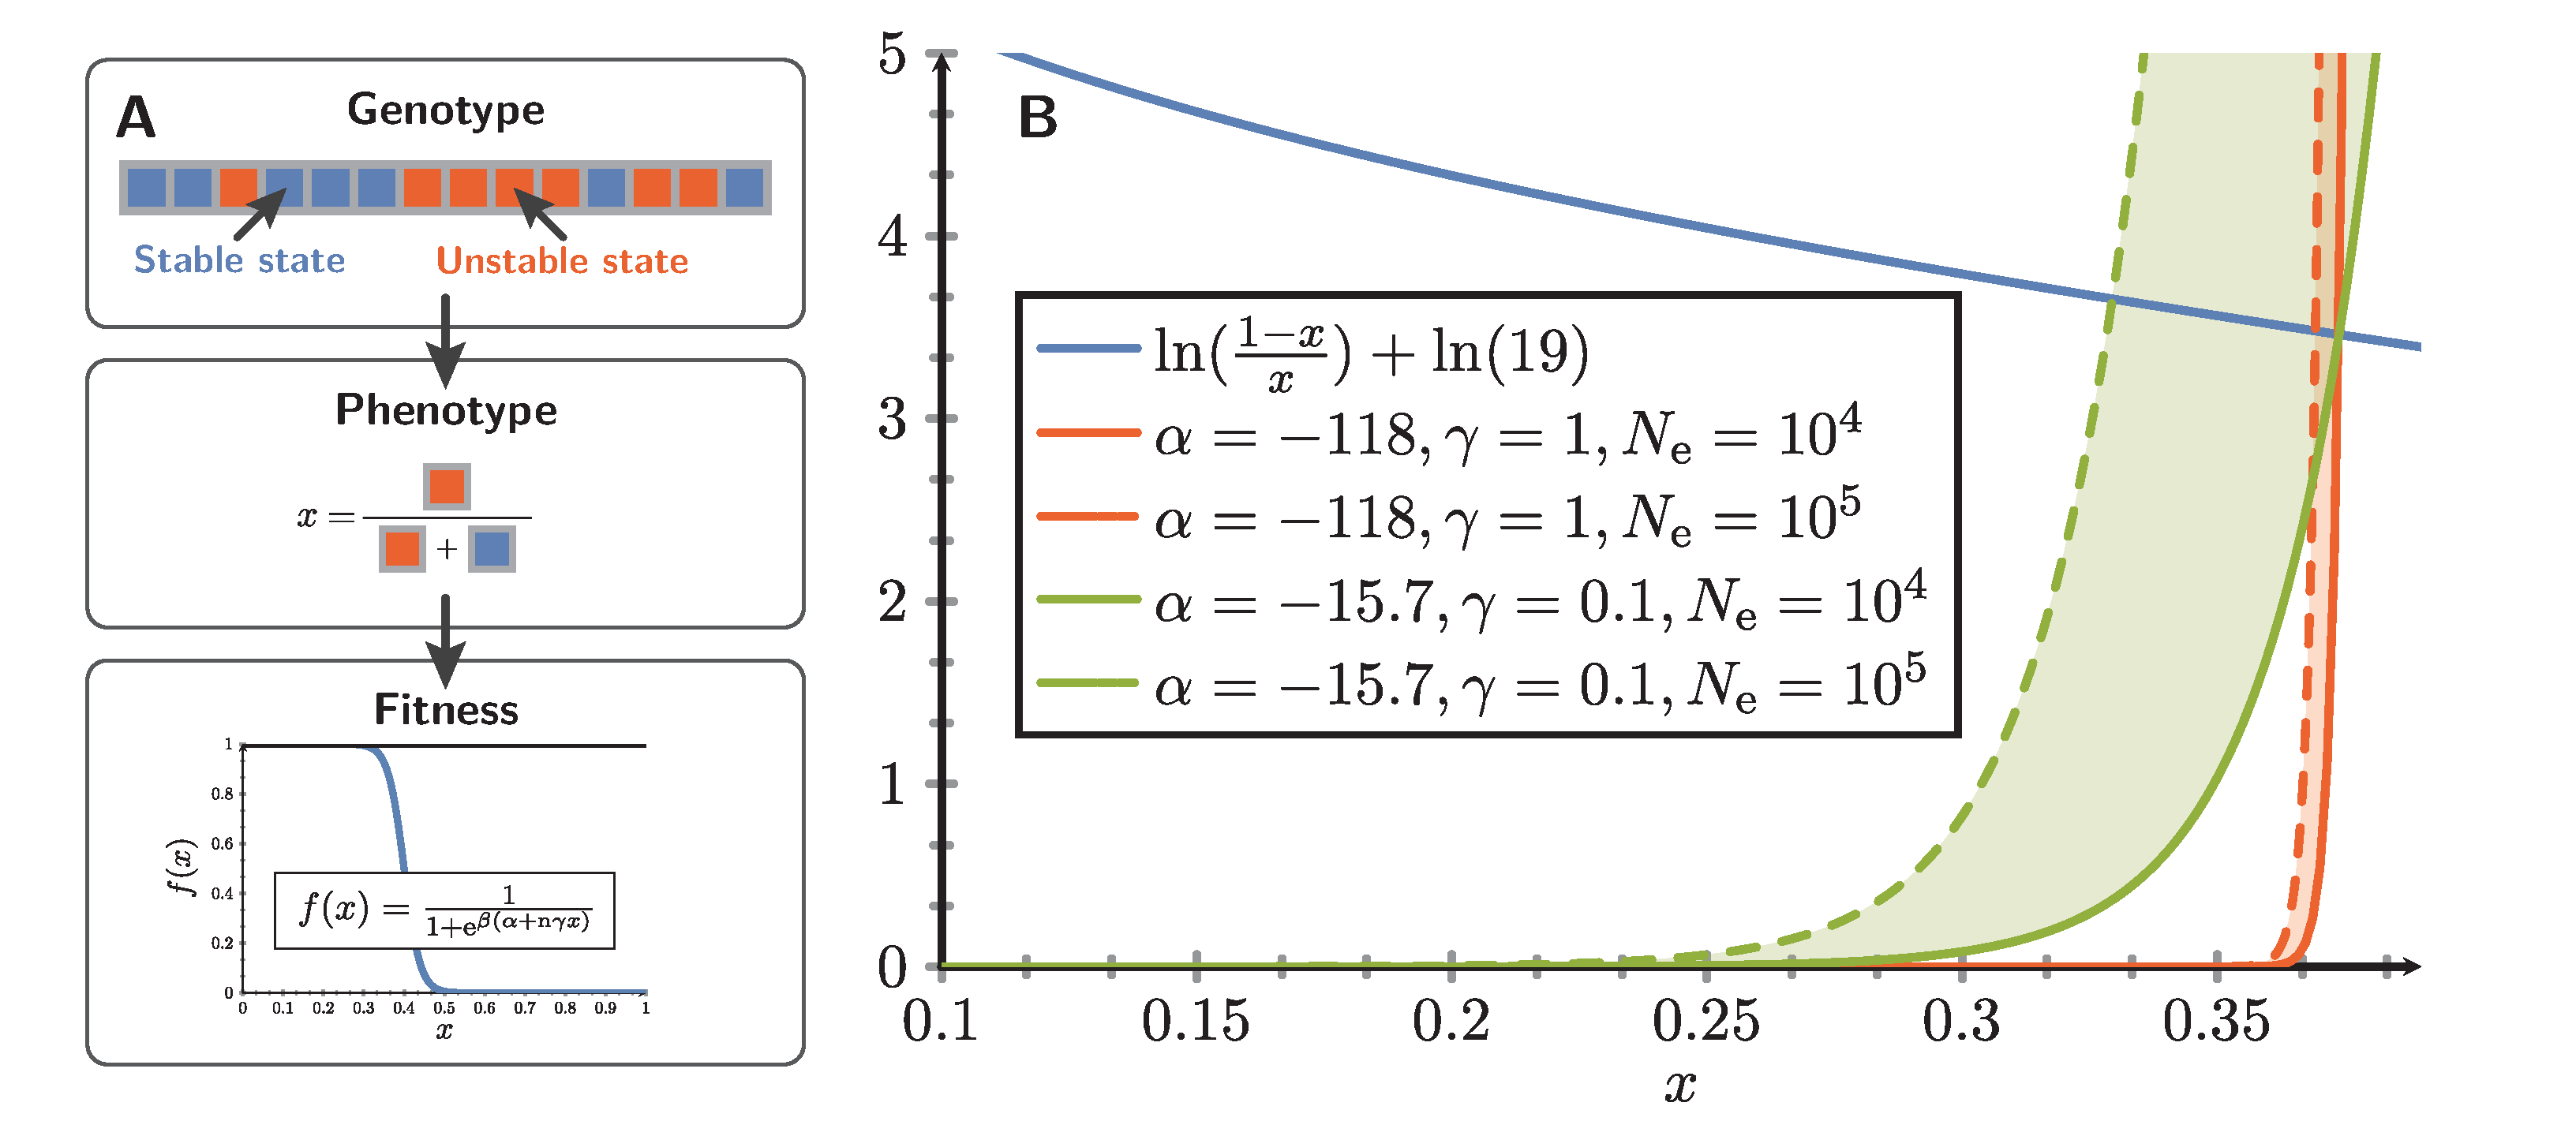
\includegraphics[width=0.9\textwidth, page=1] {artworks/theoretical.pdf}
			\caption{
				\textbf{Theoretical model.}
				Panel A. Illustration of the Genotype-phenotype-fitness map. The phenotype ($\x$) is a real-valued summary of the genotype, and is defined in our model as the fraction of unstable sites in the sequence. The fitness is a decreasing log-concave function of the phenotype.
				Panel B. Illustration of the $\dnds$ elasticity after a change in $\Ne$. The equilibrium $\x\eq$ is determined by the equation $\ln(\frac{1 - \x\eq}{\x\eq}) + \ln(19)=4\Ne \beta \gamma e^{\beta (\alpha + \Nsite \gamma \x\eq)}$. The right-hand side of the equation increases exponentially with $\x$ where $\Nsite \gamma$ is the exponential growth rate. Thus when $\Nsite \gamma$ is large (red solid line), increasing $\Ne$ (red dotted line) only changes subtly $\x\eq$ (x-axis of the crossing with the blue solid line). On the other hand, when $\Nsite \gamma$ is low (green solid line), increasing $\Ne$ (green dotted line) involve a stronger response of $\x\eq$. Moreover, changes in $\x\eq$ reflects the changes in $\dnds$ since both are related by a monotonous function (equation \ref{eq:dnds}). The value of $\alpha$ has been chosen given all other parameters such that the solid lines all cross at the same point.
			}
			\label{fig:NeChangeInfluence}
		\end{mdframed}
	\end{figure*}
	
	[Ici, manque un lien logique: the argument thus far explains how $x*$ varies with $N_e$. To capture how $\dnds$ varies with $N_e$, we also need to obtain an expression for $\dnds$ as a function of $x*$ ? quelque chose du genre?] Moreover, at equilibrium we can derive the expected substitution rate of mutations changing the sequence, and by normalizying by the substitution rate of neutral mutations, $\dnds$ simply approximates to:
	\begin{gather}
	\dnds \simeq \x\eq \label{eq:dnds}
	\end{gather}
	This simple approximation is due to substitutions at unstable sites (proportion $\x\eq$) to one of the other unstable amino-acids, which are effectively neutral and compose the largest proportion of proposed mutations with substantial probability of fixation (see equation \ref{eq:proba}).\\
	
	Finally, from the equilibrium equation \ref{eq:equilibrium}, differential calculus allow to derive the response of $\x\eq$ and ultimately $\dnds$ after a change in $\Ne$ (see supp info).
	%We define the elasticity $\chi$ as slope of the $\dnds$ response to changes in $\Ne$ in log scale, which simplify to a compact equation: 
	In the end, the elasticity of $\dnds$ to changes in $\Ne$ can be expressed in terms of a very compact equation: 
	\begin{align}
	\chi = \frac{ \der \dnds}{\der \ln (\Ne)} & \simeq - \frac{\frac{ \partial \ln f(\x\eq) }{\partial {\x\eq}}}{\frac{ \partial^2 \ln f(\x\eq) }{\partial {\x\eq}^2}}, \\
	\Rightarrow \chi & \simeq -\dfrac{1}{\beta \Nsite \gamma}.
	\end{align}
	[Ici aussi, intercaler un petit morceau de texte entre les deux équations. Par ailleurs, je me disais que ce serait utile d'interpréter un peu plus directement la version générale en termes de courbure. Je propose l'expression courbure relative pour désigner le rapport de la seconde sur la première dérivée (relative à la pente, finalement..).]
	The elasticity is thus equal to the inverse of the \emph{relative curvature}, i.e. the ratio of the second to the first derivatives, of the log-fitness function, taken at the equilibrium phenotype. Of note, this elasticity is strictly negative for decreasing log-concave fitness functions, asserting that $\dnds$ is a decreasing function of $\Ne$. In addition, the elasticity itself is low (i.e. $\dnds$ responds more weakly) for strongly concave log-fitness functions -- thus formally capturing the intuitive argument developed above (figure 1B).
	
	In the case of the biophysical model, $\chi$ is essentially independent of $\x\eq$, meaning that $\dnds$ is linearly decreasing with $\Ne$ in log scale.
	Moreover, only the compound parameter $\beta \gamma \Nsite$ has an impact on the slope of the linear relationship, where only $\gamma$ and $\Nsite$ are free parameters. [Bon, ici, il faudrait qualifier les choses: pourquoi dire que beta n'est pas un paramètre? il y a tout de même des organismes hyper-thermophiles. Par ailleurs, c'est intéressant de voir que, bien que l'équation générale semble suggérer en apparence que l'élasticité ne dépend que de la fonction de fitness, en fait, ce que montre le modèle biophysique, c'est que l'élasticité peut en réalité être modulé de deux manières: en jouant sur la relation génotype / phénotype (ici, gamma), ou en jouant sur la relation phenotype fitness (ici, beta). Raison de plus pour considérer beta comme un paramètre potentiellement libre lui aussi.]
	
	Other parametrization of the fitness function shed light on the robustness of the theoretical results.
	If the selective coefficient itself is not equal (equation \ref{eq:s-unfolded}) but proportional to the total amount of misfolded protein, and the expression level of the protein is denoted $y$, then the response of $\dnds$ to changes in $\Ne$ is the same as the response to changes in $y$ (See Supplementary Materials):
	\begin{align}
	s & \propto - \beta \gamma y  e^{\beta(\alpha + \gamma \Nsite \x)} \\
	\Rightarrow \chi = \frac{ \der \dnds}{\der \ln (y)} & \simeq -\dfrac{1}{\beta \Nsite \gamma}.
	\end{align}
	Meaning we should observe the same relationship between $\dnds$ and $\Ne$ that between $\dnds$ and expression level.\\
	
	Under empirically relevant value of $\Nsite=300$ sites and $\gamma=1.0$ kcal/mol \cite{Zeldovich2007}, the elasticity $\chi \simeq -0.002$.
	In other words, for a increase in $\Ne$ of $4$ orders of magnitude, $\dnds$ decrease approximately of $0.01$, a subtle relationship that requires laborious  effort to be detected in simulated data, and large amount of empirical data with few bias and noise to be detectable. In addition, it would imply an equally weak relation between $\dnds$ and expression level.
	
	\subsection*{Simulation experiments}
	
	In order to test the soundness of our compact theoretical results, we relaxed several assumptions by simulating DNA sequences evolution (See Methods), under various range of $\Ne$ and reporting the average $\dnds$ observed along the computation. [Là, ta phrase dit un peu tout d'un coup. Peut-être dire en plusieurs temps: Our theoretical derivation of the elasticity of $\dnds$ to changes in $N_e$ is based on several simplifying assumptions about the evolutionary model and makes multiple approximations. In order to test the robustness of our main result, we therefore conducted systematic simulation experiments, relaxing several of these assumptions. In each case, simulations were conducted under a broad range of values of $\Ne$, monitoring the average $\dnds$ observed at equilibrium and plotting the scaling of these measured equilibrium $\dnds$ as a function of $N_e$. Puis un nouveau paragraphe sur les différentes modalités qui sont relaxées.]
	
	[Specifically, with respect to mutations, our derivation assumes that... ]
	With respect to mutation, we assumed that all amino-acids transition are equiprobable, in other word the complexity of the genetic code is not taken into account.
	Simulating evolution of DNA sequence, and taking into account a matrix a mutation rate between nucleotide allow to test directly the robustness of the results to this assumption.
	Furthermore, with regards to fitness [euh non... with regards to the phenotypic effects of amino-acid changes], we assumed that all unstable [destabilizing] amino-acids are equivalently unstable [have an identical impact on protein stability. In reality, one would expect conservative amino-acid replacements to be less destabilizing than radical changes].
	This assumption is relaxed by choosing for every site of the sequence one stable amino-acid, and the impact on the phenotype ($\x$) of other amino-acids is not binary, but scaled by the Grantham amino-acid distance \cite{Grantham1974}. [Ici, ca me paraîtrait plus logique d'avoir déjà posé, même dans le modèle le plus simple, qu'en chaque position, il y a de toute manière un acide aminé optimal -- même si en pratique, sous le modèle uniforme, on n'a finalement pas besoin de préciser lequel, néanmoins, conceptuellement, le modèle ne fait de sens que parce qu'on imagine qu'il y en a un, donc ca mérite d'être déjà présent dès le début. Jj'ai proposé quelque chose en ce sens tout au début de la section résultats. Du coup, une fois que ce point est posé plus haut, alors il suffit de dire que les effets destabilisateurs en chaque position, au lieu d'être identiques pour tous les acides aminés alternatifs, sont maintenant proportionnels à la distance de Grantham entre l'acide aminé optimal en cette position et l'acide aminé proposé par la mutation non-synonyme.]
	Also [Finally], the number of sites in the sequence ($\Nsite$) is assumed to be large such that the selection coefficient is well approximated by the fitness derivative (equation \ref{eq:s}).
	The robustness of such approximation is test in the simulations with sequences of a finite number of sites ($\Nsite=300$).\\
	
	Simulations demonstrate that the relation between $\dnds$ and log-$\Ne$ is indeed linear, at least in the range explored here, and that the slope of the linear regression matches the expected theoretical value (See Figure \ref{fig:GoldsteinVsToy}, panel B [devrait toujours commencer par panel A, puis B.. quitte à inverser les panels sur ta figure]).
	Secondly we observe that the parameter $\alpha$ has virtually no effect on the slope of the linear regression, as expected also theoretically (See Figure \ref{fig:GoldsteinVsToy}, panel A). Instead, decreasing $\alpha$ (to more negative values) merely results in an overall increase in $\dnds$ over the whole range of $N_e$ (i.e. has an impact on the intercept, not on the slope). This is due to the fact that decreasing $\alpha$ shifts the equilibrium to higher $\x\eq$, since more unstable sites can then reach fixation before reaching the point of marginal stability.\\
	
	Finally, we relaxed our assumption that each site of the sequence contribute independently to $\deltaG$, by taking into account the $3$D structure of protein [and using a statistical potential to estimate $\deltaG$].
	We implemented the original model \cite{Williams2006, Goldstein2011, Pollock2012}, in which the free energy of the folded are unfolded conformations are computed using $3$D structures of the protein conformations and pairwise contact potential energies between neighboring amino-acid residues \cite{Miyazawa1985} (see Supplementary Materials).
	The original works claimed that under such $3$D model $\dnds$ is independent of $\Ne$ \cite{Goldstein2013}.
	Using extensive simulations, we argue instead that $\dnds$ is approximately linear with log-$\Ne$ (see Figure \ref{fig:GoldsteinVsToy}, panel C).
	[Ici, je dirais les choses plus diplomatiquement:
	The original works showed that under such $3$D model $\dnds$ is approximately independent of $\Ne$ \cite{Goldstein2013}.
	Using extensive simulations in order to obtain sufficient resolution, we observe that $\dnds$ is in fact weakly dependent on $N_e$, being approximately linear with log-$\Ne$ (see Figure \ref{fig:GoldsteinVsToy}, panel C).]. 
	Moreover, the observed slope matches the theoretical value considering $\deltadeltaG = 1.0$ kcal/mol for destabilizing mutations and $\Nsite=300$. 
	In such experiment, $\alpha=-118$ kcal/mol as it is the $\deltaG$ of the optimal sequence of $300$ sites \cite{Goldstein2011}.
	\begin{figure*}[htb!]
		\begin{mdframed}
			\centering
			\includegraphics[width=0.9\textwidth] {artworks/Elasticity.png}
			\caption{
				\textbf{$\bm{\dnds}$ elasticity to change in $\bm{\Ne}$}.
				For each population size, $100$ simulations were performed and the average (solid line) and $90\%$ confidence interval (shaded area) are shown.
				Panel A. The fixed parameters are $\gamma=1$, $\Nsite=300$, $\beta=1.686$, and for each non-optimal amino-acid, $\gamma$ is scaled by the Grantham distance to the optimal amino-acid. $\alpha$ are given in the legend. Decreasing $\alpha$ (to more negative values) increases $\dnds$ but changes hardly the slope of the linear regression, as expected theoretically.
				$\dnds$ at equilibrium as a function of $\bm{\Ne}$ (log scale).
				Panel B. The fixed parameters are $\Nsite=300$ and $\beta=1.686$. Parameters $\alpha$ and $\gamma$ are given in the legend.
				$\gamma$ is increased and $\alpha$ is changed accordingly such that the equilibrium value $\x\eq$ is kept constant, by solving numerically equation \ref{eq:equilibrium}.
				The slope of $\dnds$-$\Ne$ relationship decreases proportionally to the inverse of $\gamma$, as predicted by our theoretical model.
				Panel C. In the model of 3D free energy of folding, $\dnds$ at equilibrium is weakly dependent on log-$\Ne$ but is not independent as claimed originally \cite{Goldstein2013}.
				This weak dependence matches the theoretical prediction of our additive free energy model that the linear relation (dashed line) has a slope equal to $(\beta \Nsite \gamma)^{-1} = 0.00198 \simeq 0.00124$.
				Bottom D, the fixed parameters are $\alpha=-118$, $\gamma=1$, $\Nsite=300$, $\beta=1.686$, and for each non-optimal amino-acid, $\gamma$ is scaled by the Grantham distance to the optimal amino-acid.
				Moreover, with the Grantham model, the $\dnds$ matches the empirical 3D model of Golstein \& Pollock and the theoretical prediction.
				\label{fig:GoldsteinVsToy}
			}
		\end{mdframed}
	\end{figure*}
	\subsection*{Epistasis and time to relaxation}
	Although the equilibrium value of $\dnds$ after changes in $\Ne$ is an important feature of the $\dnds$-$\Ne$ relationship, another parameter that is scarcely studied is the relaxation time to reach the new equilibrium $\dnds$ \cite{Jones2016}.
	We observed in our simulations that the determining factor of the relaxation time is the number of sites $\Nsite$ (See Figure \ref{fig:relaxStability}).
	These observations match the theoretical prediction that high epistasis leads to faster return to equilibrium, since more mutational opportunities are available for driving the trait closer to equilibrium.
	More specifically, in the case of a fitness landscape with epistasis, after a change in $\Ne$, any site that contributes to pushing the trait is used to climb either up or down the fitness landscape will have diminishing return in other sites of the sequences. [Formulation pas très claire.. je me demande si la phrase juste avant ne suffit pas..]
	
	
	[Not taking into account epistasis have the consequence of overestimating the relaxation time to return to equilibrium of $\dnds$ after changes in $\Ne$ . 'overestimating' dans le contexte présent ne veut pas dire grand chose: on n'estime rien à ce stade. Par ailleurs, sauter d'un seul coup à des modèles de type mutsel site-indépendents ou DFE est un peu abrupt. Mettre en contexte. Par exemple:]
	It may be useful to compare the relaxation pattern observed here with the predictions under two alternative models of sequence evolution, representing two extreme scenarios. On one side, under a site-independent fitness landscape, such as those contemplated by many current mutation-selection models (Halpern and Bruno, Rodrigue), thus with no epistasis, every site has to adapt on its own to the new change in $\Ne$. As a result, the relaxation time is vey long, of the order of the inverse of the per-site substitution rate. On the other side, assuming a fixed distribution of fitness effect (DFE) [does not suffer from underestimating the relaxation rate - de nouveau, erreur de catégorie ici, on n'estime rien], the response of $\dnds$ is instantaneous (see Figure \ref{fig:relaxStability}).
	\begin{figure*}[htb!]
		\begin{mdframed}
			\centering
			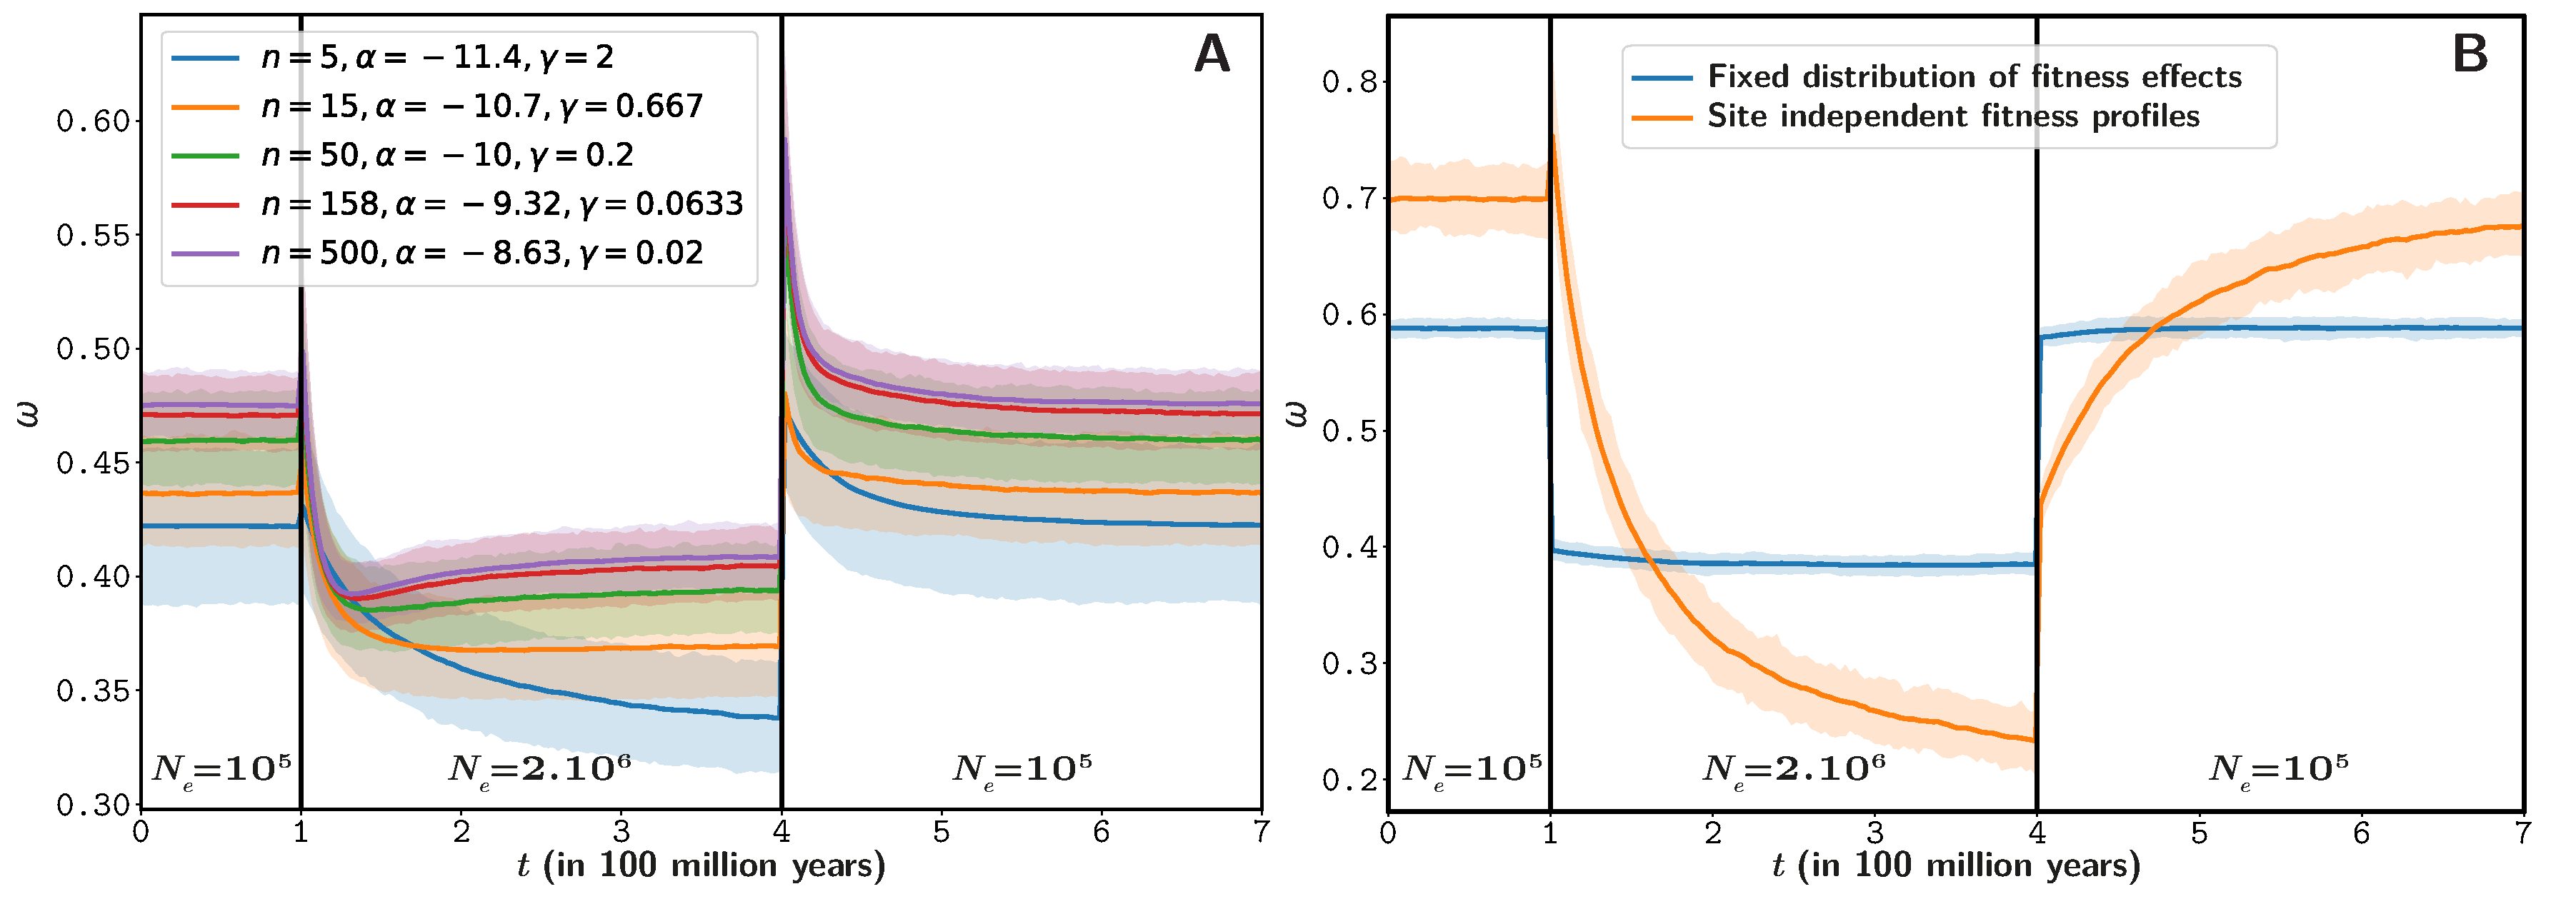
\includegraphics[width=0.9\textwidth] {artworks/Relaxation.pdf}
			\caption{
				\textbf{$\bm{\dnds}$ relaxation time to changes in $\bm{\Ne}$}.
				$\dnds$ relaxation after a brutal change in $\Ne$.
				Solid line corresponds to the average over replicates and the shaded area correspond to the $90\%$ interval among replicates. 
				The mutation rate ($\mu$) is $1e{-8}$ per year per site, and the total time of the computation is $700$ million years.
				Panel A. $\beta=1.686$, $\gamma=-10$ for all simulations. The number of sites is changed from $\Nsite=15$ to $\Nsite=158$, and the number of replicates ($r$) is changed accordingly such that the total number of sites ($\Nsite*r$) is kept constant.
				Moreover, $\gamma$ is changed according to $\Nsite$ such that the product $\gamma\Nsite$ is kept constant, thus the elasticity of the $\dnds$ to changes in $\Ne$ is kept constant.
				Finally, $\alpha$ is changed according to $\Nsite$ and $\gamma$ such that the equilibrium value $\x\eq$ is kept constant, by solving numerically equation \ref{eq:equilibrium}.
				Increasing $\Nsite$ implies a reduced time to reach the new equilibrium.
				Panel B. In context of a fixed fitness landscape, where each amino-acid has different fitness (site-specific profile), the time taken to reach the new equilibrium value of $\dnds$ after a change in $\Ne$ is long, such that relaxation rate is on the order of the mutation rate. In the context of a distribution of fitness effects, the relaxation time is non-existent.
			}
			\label{fig:relaxStability}
		\end{mdframed}
	\end{figure*}
	
	[L'ensemble du paragraphe ci-dessous me semble plus être de la discussion - par ailleurs, il faudrait le retravailler un peu]
	Previous studies have argued that model of protein evolution should consider epistasis for various empirical reasons such as rate heterogeneity along the sequence, rate and time dependence of convergence, role of compensatory substitutions, prediction of deleterious mutations \cite{Goldstein2017}.
	We argue that epistasis also has an important role in the non-stationary response of $\dnds$ to changes in $\Ne$ [attention: on a précédemment défini l'elasticité comme la réponse du omega d'équilibre à des changements de log Ne, on ne peut donc pas parler d'élasticité hors équilibre comme cela. Je n'utiliserais pas ce terme dans ce contexte].
	If epistasis is not taken into account, the relaxation time of $\dnds$ is incompatible with biological evolution [phrase un peu abrupte, telle quelle: incompatble avec quoi exactement?].
	
	
	
	\section*{Discussion}
	The negative relationship between the relative substitution rate of selected mutations ($\dnds$) and $\Ne$ has been predicted theoretically under the quasi-neutral theory of evolution.
	Empirical data showed mitigated confirmation of this prediction, encouraging alternative explanatory mechanism.
	One such explanation, developed in the context of genotype-phenotype-fitness map, demonstrated the absence of $\dnds$ elasticity to changes in $\Ne$ if the probabilities of phenotype changes are invariant to the current phenotype.
	We argue that this assumption can be relaxed, and provide theoretical tools to derive the relationship between $\Ne$ and $\dnds$ in this context.
	We apply our framework in the special case of fitness proportional to the proportion of folded proteins. \\
	% Goal and theoretical results
	
	Our theoretical results demonstrate that the relationship between $\dnds$ and $\Ne$ (in log space) is linear with a negative slope.
	This slope is a function of molecular parameters of the model, and is inversely proportional to the product of the sequence size and the average change in conformational energy of destabilizing mutations. 
	Based on empirical estimate of the molecular parameters, the elasticity of $\dnds$ to changes in $\Ne$ would be $\chi \simeq 0.002$.
	Our compact theoretical results are supported by more complex simulations of protein evolution relaxing several assumptions.
	% Our theoretical results are robsut to approximations
	
	Particularly, our theoretical prediction match a numerical model of protein evolution, in which the free energy of the folded are unfolded conformations are computed using $3$D structures of the protein conformations.
	Previous studies using this model presented an apparent lack of $\dnds$ elasticity to changes in $\Ne$ \cite{Goldstein2013}.
	We argue the apparent lack of elasticity is in fact due to the subtle relation, and require extensive computation to be detected.\\
	% Goldstein \& Pollock model don't have a null elasticity
	
	Empirically, inference of the $\dnds$ elasticity in Primates, using polymorphism and divergence data estimated $\chi \simeq $, approximately $X$ times greater than our theoretical prediction \cite{Brevet2019}.
	More empirical data across clades would be required to infirm such model, but in the light of empirical data estimating the relationship between $\Ne$ and $\dnds$, models based on the probability of folding are not reasonably fitted.\\
	% Our result show the fitness proportional to proportion of folded folding is at odd with empirical data
	
	Furthermore, our theoretical results manifest that the relationship between $\Ne$ and $\dnds$ is the same as the relationship between protein abundance and $\Ne$, whenever protein fitness is determined by the deleterious effect of unfolded proteins.
	As such, dataset relating $\dnds$ to $\Ne$ and protein can be used confirm or infirm this model.\\
	% Stress the importance that elasticity is valid for Ne and protein abondance
	
	Notably, theoretical approximations apply more broadly to protein-protein interactions (See Supplementary Materials), where protein may either be in free form or engaged in a non-specific interaction. 
	In non-specific interactions, stable site are hydrophilic amino-acid and unstable site are hydrophobic amino-acid at the protein surface.
	Fitting this model with empirical estimates \cite{Zhang2008}, we obtain an elasticity of $\chi = 0.2$ (See Supplementary Materials) thus a much stronger response than under the model based on conformational stability. 
	This effect is due to less sites in the protein being involved in protein-protein interaction than for conformational stability, in addition to the lower energy engaged in the contacts.
	As such, in light of empirical data available, the assumption that protein fitness is determined such as to avoid non-specific interaction is more likely than the assumption that protein fitness is determined by the deleterious effect of unfolded proteins. \\
	% Protein-protein interactions
	
	% DFE can also be used to fit to empirical data - Shall we present this ?
	
	\section*{Materials \& Methods}
	Protein sequence evolution is simulated under an origin-fixation model \cite{McCandlish2014}, where one sequence represent the whole population.
	From the resident DNA sequence $\ci$, we define $\setNeighbors$ as the set of all possible mutant that are one nucleotide away from $\ci$, and were mutant sequences containing a stop codon are excluded.
	For a protein of $\Nsite$ amino-acid sites, $\left| \setNeighbors \right| \leq 9 \Nsite$, since each codon has a maximum of $9$ possible mutant codons that are one mutation away and that are not stop codon.
	For each mutant sequence $\cj \in \setNeighbors$, we compute its fitness and subsequently the selection coefficient of the mutant:
	\begin{equation}
	s \left( \ci,\cj\right) = \dfrac{ f \left(\cj \right) - f \left(\ci\right) }{f\left( \ci \right)}.
	\end{equation}
	The next event of mutant invading the population, and the time to reach such event is chosen using Gillespie algorithm, according to the rates of substitution between sequences:
	\begin{equation}
	\submatrix_{\itoj} = \mu_{\itoj} \dfrac{4 \Ne s \left( \ci,\cj\right)}{1 - \e^{-4 \Ne s \left( \ci,\cj\right)}}, 
	\end{equation}
	where $\mu_{\itoj}$ is the mutation rate between $\ci$ and $\cj$, determined by the underlying $4x4$ nucleotide mutation rate matrix, and ${\submatrix_{\itoj}} = \mu_{\itoj}$ in the case of synonymous substitutions.
	Various optimization are implemented to reduce the computation time of mutant's fitnesses.
	The simulation starts with a burn-in period to reach mutation-selection-drift equilibrium.
	\subsection*{Models of fitness function}
	\label{MatMet:folding}
	Under a simulation of protein folding with an additive model of free energy, the protein's difference in free energy between folded and unfolded state is given by:
	\begin{equation*}
	\deltaG\left(\ci\right) = \alpha + \Nsite \gamma * \x\left(\ci\right), 
	\end{equation*}
	where $0 \leq \x\left(\ci\right) \leq 1$ is the distance of $\ci$ to the optimal sequence.
	For each site of sequence, the optimal amino-acids are chosen randomly at initialization, and the distance between the current amino-acid and the optimal is scaled by the Grantham amino-acid distance \cite{Grantham1974}.
	Wrightian fitness is defined as the probability of our protein to be in the folded state, given by the Fermi-Dirac distribution: 
	\begin{equation}
	f(\deltaG\left(\ci\right)) = \dfrac{e^{-\beta \deltaG\left(\ci\right) }}{1 + e^{-\beta \deltaG\left(\ci\right) }} = \dfrac{1}{1 + e^{\beta \deltaG\left(\ci\right) }}, 
	\end{equation}
	where $\beta$ is the inverse of the temperature ($\beta=1/kT$).\\
	
	Under a simulation with site independent fitness profiles, a fitness profile give a fitness for each amino-acid (vector of size $20$).
	Each site of the protein has a specific amino-acid fitness profile.
	Overall, the protein phenotype is computed as the sum of site-specific selection coefficient, obtained by accessing the amino-acid present at each site of the protein.
	The selection coefficient of the mutant $\cj$ is:
	\begin{equation}
	s \left( \ci,\cj\right) = \sum_{1 \leq \site \leq \Nsite} \ln \left( \dfrac{G_{\site} \left(\cj(\site) \right)}{G_{\site} \left(\ci(\site) \right)} \right) ,
	\end{equation}
	where $G_{\site}$ is the fitness profile at site $\site$, obtained in empirical experiment \cite{Bloom2017}.
	
	
	Under simulation with a fixed distribution of fitness effects (DFE), the selection coefficient of the mutant $\cj$ is gamma distributed (shape $\beta > 0$):
	\begin{equation}
	- s \left( \ci,\cj\right) \sim \text{Gamma} \left( \bar{|s|}, \beta \right)
	\end{equation}
	\subsection*{$\bm{\dnds}$ along the simulation}
	From the set of mutants $\setNeighbors$ that is one nucleotide away from $\ci$, we define the subsets $\setNonSynNeighbors$ and $\setSynNeighbors$ that are respectively the set of non-synonymous and synonymous mutants, where $\setNonSynNeighbors \cup \setSynNeighbors = \setNeighbors$.
	As in previous works \cite{Spielman2015a, DosReis2015, Jones2016}, the ratio of non-synonymous over synonymous substitution rates of the sequence is defined as :
	\begin{align}
	\dnds(t) &= \dfrac{\sum_{\cj \in \setNonSynNeighbors} \submatrix_{\itoj}}{\sum_{\cj \in \setNonSynNeighbors} \mu_{\itoj}} \left( \dfrac{\sum_{\cj \in \setSynNeighbors} \submatrix_{\itoj}}{\sum_{\cj \in \setSynNeighbors} \mu_{\itoj}} \right)^{-1}\\
	&= \dfrac{\sum_{\cj \in \setNonSynNeighbors} \mu_{\itoj} \dfrac{4 \Ne s \left( \ci,\cj\right)}{{1 - \e^{-4 \Ne \left( \ci,\cj\right)} }}}{\sum_{\cj \in \setNonSynNeighbors} \mu_{\itoj}} 
	\end{align}
	And $\dnds$ is taken as the average of the time-dependent $\dnds(t)$ along the simulation.
	\subsection*{Reproducibility}
	The simulators written in C++ are publicly available under MIT license at \url{https://github.com/ThibaultLatrille/SimuEvol}.
	The scripts and instructions necessary to reproduce the experiments are available at \url{https://github.com/ThibaultLatrille/GenotypePhenotypeFitness}.
	\bibliographystyle{apalike}
	\bibliography{refs-codons,refs-cds}
	
\end{document}